\documentclass[english,12pt,a4paper]{beamer}
\usepackage[T1]{fontenc}
\usepackage{babel}
\usepackage{geometry}
\usepackage{hyperref}
\hypersetup{
	hidelinks=true,
	colorlinks=true,
	linkcolor=black,
	filecolor=magenta,      
	urlcolor=blue,
	pdftitle={Final Project},
	pdfpagemode=FullScreen,
}
\usepackage{amsmath}
\usepackage{multirow}
\usepackage{pgfplots}
\usepackage{xcolor}
\usepackage{listings}
\lstdefinestyle{mystyle}{
	commentstyle=\color{green},
	keywordstyle=\color{blue},
	%	numberstyle=\tiny\color{codegray},
	stringstyle=\color{magenta},
	basicstyle=\ttfamily\footnotesize,
	breakatwhitespace=false,         
	breaklines=true,                 
	captionpos=t,                    
	keepspaces=true,
	tabsize=2,
	prebreak=\raisebox{0ex}[0ex][0ex]{\ensuremath{\hookleftarrow}}
}

\lstset{style=mystyle}
\usepackage{multimedia}


% Computation of Trajectory in Two-Body Problem
% Numerical Solution of Two-Body Problem
\title{Numerical Methods for Solving Ordinary Differential Equations in Two-Body Problem}

\author{Kamil Chaj}



\date{2023/2024}
\begin{document}
	\frame{\titlepage}
	\graphicspath{ {../latex/pictures/} }
	
	\begin{frame}
		\frametitle{Two-body problem}
		\begin{itemize}
			\item in system there exists only two bodies
			\item bodies have uniform mass distributions and are perfectly symmetrical
		\end{itemize}
	\end{frame}
	
	\begin{frame}
		\frametitle{Two-body problem}
			\centering
			$$
			\vec{r_0} = \vec{r_2} - \vec{r_1}
			$$
			
			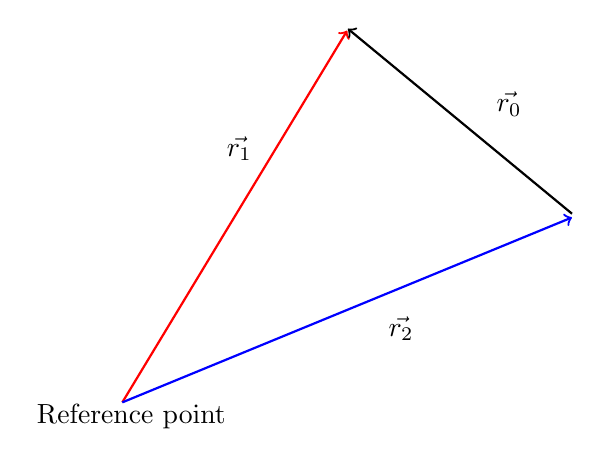
\begin{tikzpicture}
				
				\begin{axis}[
					hide axis,
					clip=false
					]
					\addplot[
					->, thick, red
					] coordinates {
						(0, 0) (2.99, 1.99) 
					};
					\addplot[
					->, thick, blue
					] coordinates {
						(0, 0) (5.98, 0.99)
					};
					\addplot[
					->, thick
					] coordinates {
						(5.98, 1.01) (3, 2) 
					};
					\node[above] at  (axis description cs:0.8,0.7) {$\vec{r_0}$};
					\node[above] at  (axis description cs:0.3,0.6) {$\vec{r_1}$};
					\node[above] at  (axis description cs:0.6,0.2) {$\vec{r_2}$};
					\node[below] at  (axis description cs:0.1,0.1) {Reference point};
					
%					\addplot [mark=*,nodes near coords,only marks,point meta=explicit symbolic]
%					table[meta=label] {
%						x   y   label
%						3   2   $m_1$
%						6   1	$m_2$
%					};					
				\end{axis}
			\end{tikzpicture}
	\end{frame}
	\begin{frame}
		\frametitle{Derivation}
		\begin{equation}\label{gen_tb}
			\begin{cases}
				m_1 \frac{d^2\vec{r_1}}{dt^2} = \vec{F} \\
				m_2 \frac{d^2\vec{r_2}}{dt^2} = - \vec{F} \\
			\end{cases}
		\end{equation}
		\begin{equation}\label{uni_newton}
			\vec{F} = G \frac{m_1 m_2}{r_0^2}\hat{r_0}, \qquad \hat{r_0} = \frac{\vec{r_0}}{r_0}
		\end{equation}
		\begin{equation}\label{vec}
			\vec{r_0} = \vec{r_2} - \vec{r_1}
		\end{equation}
	\end{frame}
	\begin{frame}
		\frametitle{Derivation}
		\begin{equation}
			\begin{cases}
				\dfrac{d^2\vec{r_1}}{dt^2} =  \dfrac{G m_2}{||\vec{r_2} - \vec{r_1}||^3} (\vec{r_2} - \vec{r_1})\\
				\dfrac{d^2\vec{r_2}}{dt^2} =  \dfrac{G m_1}{||\vec{r_2} - \vec{r_1}||^3} (\vec{r_1} - \vec{r_2})
			\end{cases}
		\end{equation}	
	\end{frame}
	
	\begin{frame}
		\frametitle{Initial conditions}
			\begin{equation}
			\begin{bmatrix}
				\vec{r_1}(t_0) \\ \vec{r_2}(t_0) \\ \vec{v_1}(t_0) \\ \vec{v_2}(t_0)
			\end{bmatrix}
			=
			\begin{bmatrix}
				x_1(t_0) & y_1(t_0) & z_1(t_0)\\
				x_2(t_0) & y_2(t_0) & z_2(t_0)\\
				v_{x1}(t_0) & v_{y1}(t_0) & v_{z1}(t_0)\\
				v_{x1}(t_0) & v_{y1}(t_0) & v_{z1}(t_0)
			\end{bmatrix}
			, \qquad t_0 = 0
		\end{equation}
	\end{frame}
	
	\begin{frame}
		\frametitle{In MATLAB}
		\lstinputlisting[language=matlab,numbers=left]{../matlab/base_ode.m}
	\end{frame}
	
	\begin{frame}
		\frametitle{Idea behind numerical methods}
		\begin{equation}\label{eq:num}
			\frac{d \vec{v}}{dt} = f(\vec{r}, t) \implies \frac{\Delta \vec{v}}{\Delta t} = f(\vec{r}, t_n)
		\end{equation}
		\begin{equation}
			\Delta \vec{v} = f(\vec{r}, t_n) \Delta t = f(\vec{r}, t_n) h
		\end{equation}
		$$
			\Delta t = h
		$$
	\end{frame}
	
	\begin{frame}
		\frametitle{Euler method}
		\begin{equation}
			\begin{split}
				\vec{r_{n+1}} &= \vec{r_{n}} + \Delta \vec{r} \\
				&= \vec{r_{n}} + f(\vec{r_n}, t_{n + 1 }) h
			\end{split}
		\end{equation}
		
		\begin{equation}
			\begin{bmatrix}
				\vec{r_{n+1}}\\
				\vec{v_{n+1}}\\
			\end{bmatrix}
			=
			\begin{bmatrix}
				r_n + v_n h\\
				v_n + f(\vec{r_n}, t_{n+1}) h
			\end{bmatrix}
		\end{equation}
	\end{frame}
	
	\begin{frame}
		\frametitle{In MATLAB}
		\lstinputlisting[language=matlab,numbers=left]{../matlab/euler.m}
	\end{frame}
	
	\begin{frame}
		\frametitle{4th order Runge-Kutta method}
		\begin{equation}\label{eq:RK4}
			\begin{split}
				k_1 &= f(\vec{r_n},  t_0 + n h)\\
				k_2 &= f\left(\vec{r_n} + k_1 \frac{h}{2}, t_0 + h(n + \frac{1}{2})\right)\\
				k_3 &= f\left(\vec{r_n} + k_2 \frac{h}{2}, t_0 + h(n + \frac{1}{2})\right)\\
				k_4 &= f\left(\vec{r_n} + k_3 h, t_0 + h(n + 1)\right)
			\end{split}
		\end{equation}
		\begin{equation}
			\vec{v_{n+1}} = \vec{v_n} + \frac{h}{6}(k_1 + 2 k_2 + 2k_3 + k_4)
		\end{equation}
		\begin{equation}
			\begin{bmatrix}
				\vec{r_{n+1}}\\
				\vec{v_{n+1}}\\
			\end{bmatrix}
			=
			\begin{bmatrix}
				r_n + v_n h\\
				v_n + \frac{h}{6}(k_1 + 2 k_2 + 2k_3 + k_4)
			\end{bmatrix}
		\end{equation}
	\end{frame}
	
	\begin{frame}
		\frametitle{In MATLAB}
		\lstinputlisting[language=matlab,numbers=left,basicstyle={\scriptsize }]{../matlab/RK4.m}
	\end{frame}
	
	\begin{frame}
		\frametitle{Convergence analysis}
		\begin{equation}
			S_C(R_{n-1}, R_{n}) = \cos(\theta) = \dfrac{\langle \vec{R_{n-1}}, \vec{R_{n}} \rangle}{R_{n-1} R_{n}}
		\end{equation}
		
		\begin{equation}
			D_\theta (R_{n-1}, R_{n}) = \arccos(S_C(R_{n-1}, R_{n})) = \theta
		\end{equation}
	\end{frame}
	
	\begin{frame}
		\begin{figure}[h!]
			\centering
			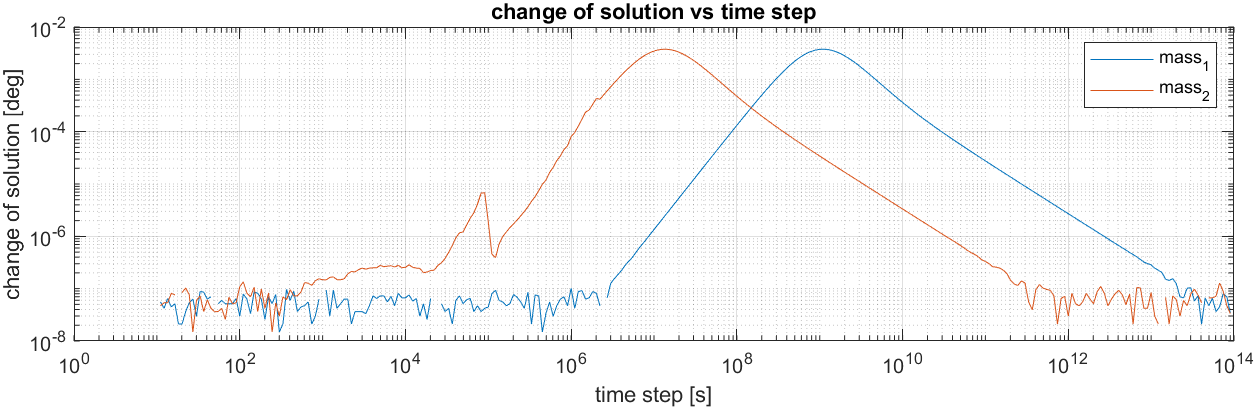
\includegraphics[width = 0.9\textwidth]{euler_err.png}
			\caption{\scriptsize Euler method}
		\end{figure}
		
		\begin{figure}[h!]
			\centering
			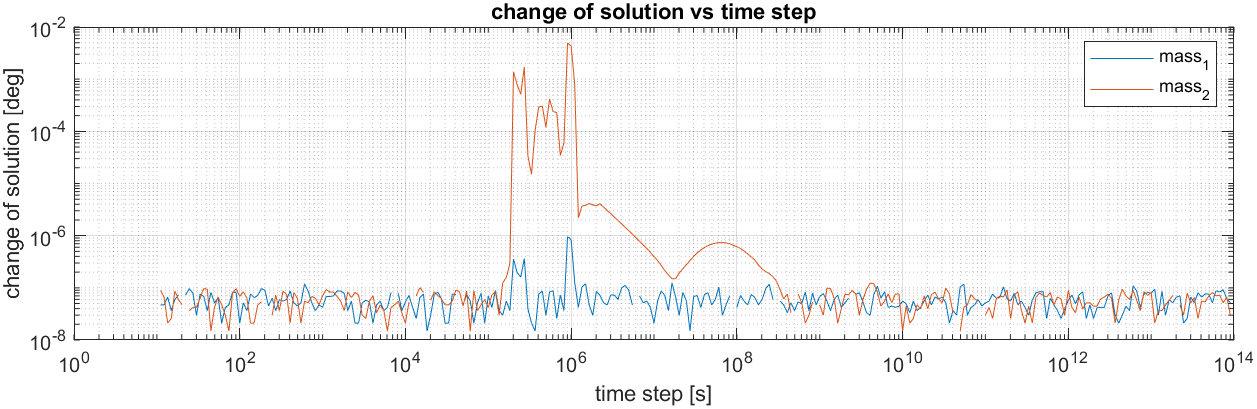
\includegraphics[width = 0.9\textwidth]{RK4_err.png}
			\caption{\scriptsize Runge-Kutta method}
		\end{figure}
		
	\end{frame}
	
	\begin{frame}
		\frametitle{in MATLAB}
		\lstinputlisting[language=matlab,numbers=left,basicstyle={\scriptsize }]{../matlab/err_test_p.m}
	\end{frame}
	
	\begin{frame}
		\frametitle{Computation time}
		\begin{figure}[h!]
			\centering
			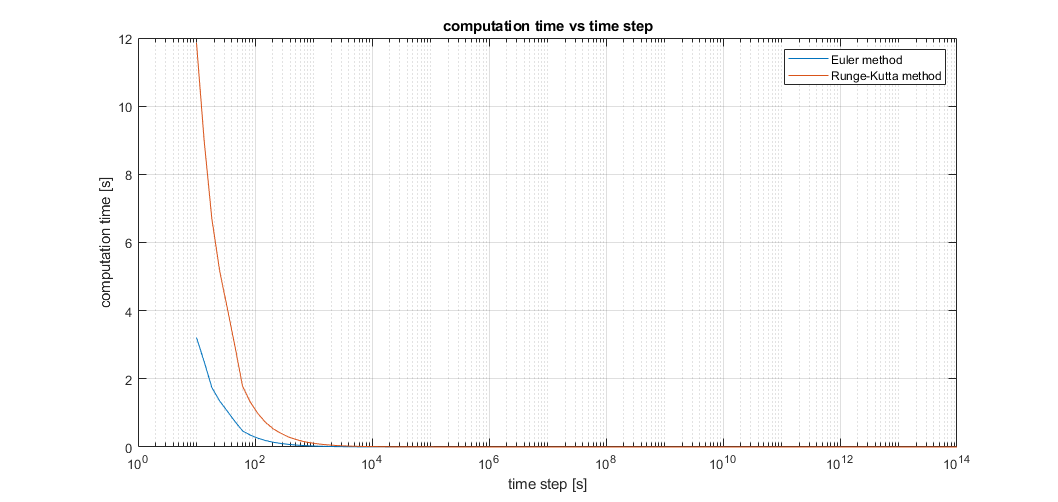
\includegraphics[width = 0.9\textwidth]{time_comp.png}
			\caption{Comparison of computation time between methods}
		\end{figure}
	\end{frame}
	
	\begin{frame}
		\frametitle{in MATLAB}
		\lstinputlisting[language=matlab,numbers=left]{../matlab/comp_time_p.m}
	\end{frame}
	
	\begin{frame}
		\Large Demo
	\end{frame}
		
\end{document}